\documentclass{beamer}
\mode<presentation>
\usetheme{CambridgeUS}
\usepackage[russian]{babel}
\usepackage[utf8]{inputenc}
\usepackage[T2A]{fontenc}
\usepackage{sansmathaccent}

\usepackage{verbatim}
\usepackage{alltt}

\pdfmapfile{+sansmathaccent.map}
\title[Язык C]{Основы программирования на С}
\author{Наумов Д.А., доц. каф. КТ}
\date[11.02.2019] {Операционные системы и системное программное обеспечение, 2019}

\begin{document}

%ТИТУЛЬНЫЙ СЛАЙД
\begin{frame}
  \titlepage
\end{frame}
  
%СОДЕРЖАНИЕ ЛЕКЦИИ
\begin{frame}
  \frametitle{Содержание лекции}
  \tableofcontents  
\end{frame}

\section{Краткая характеристика языка}

\begin{frame}{Краткая характеристика языка}
Язык Си – язык программирования высокого уровня, разработанный Д.Ритчи и его коллегами в 70х гг прошлого века. Он представляет собой минималистичный процедурный язык программирования, в котором упор сделан на эффективность компиляции.
\begin{itemize}
\item многие возможности вынесены из базовых средств языка и предоставляются стандартной библиотекой, при этом прототипы и семантика функций стандартной библиотеки фиксированы и не зависят от конкретного компилятора, вместе с которым она поставляется;
\item Си часто называют «высокоуровневым ассемблером», поскольку он предоставляет возможность писать эффективные программы с весьма низким уровнем абстракции;
\item Си не привязан к конкретной аппаратуре или операционной системе и предназначен для написания машинно-независимых и легко переносимых программ.
\end{itemize}
\end{frame} 

\section{Базовые типы данных}
\begin{frame}{Базовые типы даных}
\begin{itemize}
\item Базовые типы: char, int, float и double;
\item Квалификаторы: short, long, signed и unsigned.
\item Конкретные размеры типов определяются реализацией компилятора.
\end{itemize}
\end{frame} 

\begin{frame}{Переменные и константы}
\begin{itemize}
\item Имена переменных могут состоять из букв (знак подчеркивания считается буквой) и цифр. Первая литера обязательно буква;
\item Большие и маленькие буквы различаются.
\item Для внутренних имен значимыми являются первые 31 литера, а для внешних – 6 литер.
\item Все переменные должны быть описаны до использования.
\end{itemize}
\begin{figure}[h]
\centering
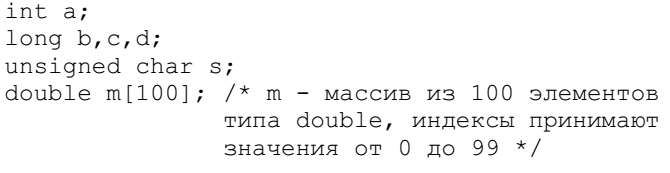
\includegraphics[scale=0.6]{images/lec02-pic01.png}
\end{figure}
\end{frame}

\begin{frame}{Константы}
\begin{itemize}
\item квалификатор const - значение переменной не будет изменяться;
\item целые константы: 123, 017, 0x1a, 0X1A, 123L, 1024U
\item вещественные константы (double): 123.4, 1.234e2, 123.4L
\item вещественные константы (float): 123.4f, 1.234e2f
\item символьные константы: '*', 's', '$\setminus n$', '$\setminus t$', '$\setminus 123$', '$\setminus x12$'
\item строковые константы: "asdf"  неявно заканчивается '$\setminus 0$'
\end{itemize}
\begin{figure}[h]
\centering

\includegraphics[scale=0.6]{images/lec02-pic02.png}
\end{figure}
\end{frame}

\begin{frame}{Перечислимый тип}
\begin{figure}[h]
\centering
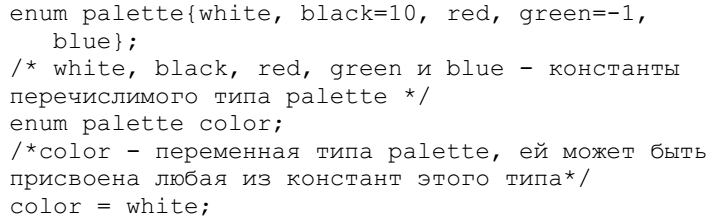
\includegraphics[scale=0.6]{images/lec02-pic03.png}
\end{figure}
\begin{itemize}
\item именование констант перечислимого типа уникально в пределах области видимости;
\item константы ассоциированы с целым типом Си и могут использоваться везде, где используются константы типа int;
\item по умолчанию, константам перечислимого типа присваиваются последовательные значения (0,1,2, ….).
\end{itemize}
\end{frame}

\section{Операции над базовыми типами данных}
\begin{frame}{Операции над базовыми типами}
\begin{block}{Арифметические операции (+, -, *, /, \%)}
\begin{itemize}
\item унарные операции + и - (изменяет знак стоящей справа величины) имеют более высокий приоритет, чем бинарные операции + и - ;
\item бинарные операции +(сложение) и –(вычитание) имеют одинаковый приоритет, он ниже приоритета операций
*(умножение), /(деление) и \%(остаток от деления);
\item операция / с операндами целых типов выполняется с усечением дробной части;
\item операция \% определена только для операндов целых типов;
\item арифметические операции с одинаковым приоритетом выполняются слева направо
\end{itemize}
\end{block}
\end{frame}

\begin{frame}{Операции над базовыми типами}
\begin{block}{Логические операции (!, \&\&, ||)}
\begin{itemize}
\item результатом унарной операции !(логическое НЕ) будет 0 для ненулевого операнда и 1 для нуля;
\item приоритет бинарной операции \&\&(логическое И) выше приоритета бинарной операции ||(логическое ИЛИ).
\end{itemize}
\end{block}
\end{frame}

\begin{frame}{Операции над базовыми типами}
\begin{block}{Операции отношения(<, <=, >, >=, ==, !=)}
\begin{itemize}
\item операции <, <=, >, >= имеют одинаковый приоритет, он ниже приоритета операций сравнения на равенство == и != ;
\item операции отношения имеют более низкий приоритет, чем арифметические операции, но более высокий, чем логические операции \&\& и ||.
\end{itemize}
\end{block}
\end{frame}

\begin{frame}{Операции над базовыми типами}
\begin{block}{Инкрементная и декрементная операции}
\begin{itemize}
\item могут быть как префиксными, так и постфиксными, так, например, ++x увеличивает x на 1 до того, как его значение будет использовано, а x++ - после;
\item эти операции можно применять только к переменным: запись ++(x+y) не верна.
\end{itemize}
\end{block}
\end{frame}

\begin{frame}{Операции над базовыми типами}
\begin{block}{Условная(тернарная) операция (?:)}
\begin{itemize}
\item в выражении x?y:z первым вычисляется значение выражения x, и если оно не равно нулю, то результатом всей операции будет значение выражения у, иначе – значение выражения z.
\end{itemize}
\end{block}
\end{frame}

\begin{frame}{Операции над базовыми типами}
\begin{block}{Побитовые операции \& , |, $<<$, $>>$, $\sim$, $\wedge$}
\begin{itemize}
\item все побитовые операции можно применять только к операндам целых типов (знаковым и беззнаковым char, short, int и
long);
\item результат поразрядных операций \& и | не совпадает с результатом логических операций \&\& и ||, например, для x=2 и y=5 результатом x\& y будет 0, тогда как результатом x\&\& у будет 1;
\item операции $<<$(сдвиг влево) и $>>$(сдвиг вправо) могут использоваться как эффективное умножение и деление на степени 2
\end{itemize}
\end{block}
\end{frame}

\begin{frame}{Приведение типов}
\begin{figure}[h]
\centering
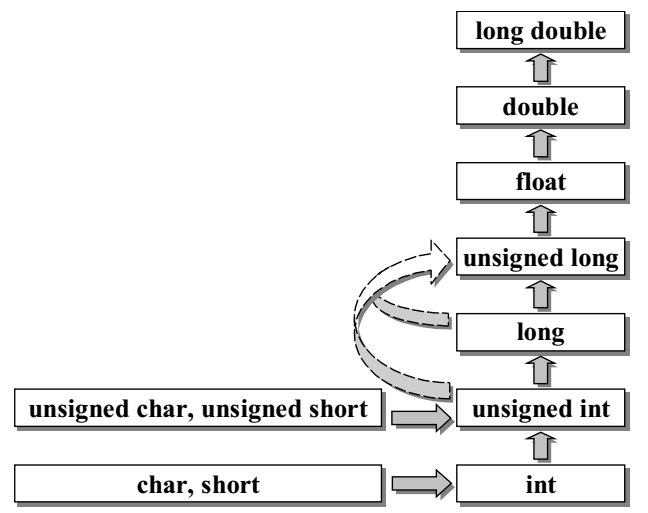
\includegraphics[scale=0.5]{images/lec02-pic04.png}
\end{figure}
\end{frame}

\begin{frame}{Приведение типов}
Пример 1
\begin{figure}[h]
\centering
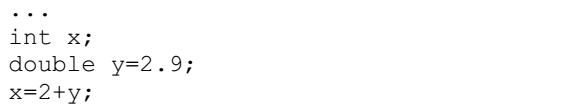
\includegraphics[scale=0.5]{images/lec02-pic05.png}
\end{figure}
Пример 2
\begin{figure}[h]
\centering

\includegraphics[scale=0.5]{images/lec02-pic06.png}
\end{figure}
\end{frame}

\section{Операторы управления}
\begin{frame}{Операторы управления}
Программа на языке Си состоит из набора функций.
\begin{itemize}
\item При запуске программы на выполнение управление передается на точку входа в функцию с названием main.
\item Функции состоят из операторов. 
\item Выражение становится оператором, если за ним идет точка с запятой. 
\item Точка с запятой заканчивает любой оператор, кроме составного оператора { }
\end{itemize}
\begin{block}{Операторы}
\begin{itemize}
\item присваивания
\item условный оператор (оператор if)
\item оператор выбора (переключатель switch)
\item оператор цикла с предусловием (while)
\item оператор цикла с постусловием (do-while)
\item оператор цикла с параметром (for)
\item операторы break и continue
\end{itemize}
\end{block}
\end{frame} 

\begin{frame}
Пример 3. Из стандартного входного потока ввести строку и записать ее в массив str. Длина строки не превышает 80 символов. 
\begin{figure}[h]
\centering
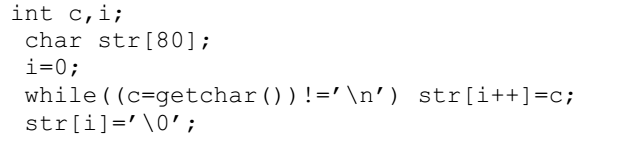
\includegraphics[scale=0.5]{images/lec02-pic07.png}
\end{figure}
\end{frame}

\begin{frame}
Пример 4. Обнуление элементов одномерного массива. 
\begin{figure}[h]
\centering
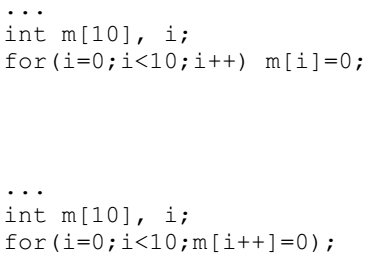
\includegraphics[scale=0.5]{images/lec02-pic08.png}
\end{figure}
\end{frame}

\begin{frame}
Пример 5. Определение длины строки. 
\begin{figure}[h]
\centering
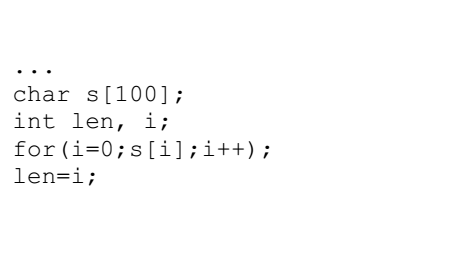
\includegraphics[scale=0.5]{images/lec02-pic09.png}
\end{figure}
\end{frame}

\begin{frame}
Пример 6. 
\begin{figure}[h]
\centering
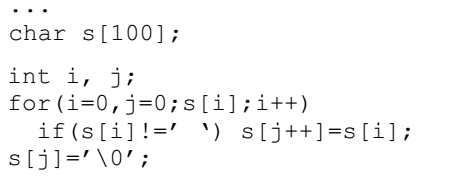
\includegraphics[scale=0.5]{images/lec02-pic10.png}
\end{figure}
\end{frame}

\begin{frame}
Пример 7. 
\begin{figure}[h]
\centering
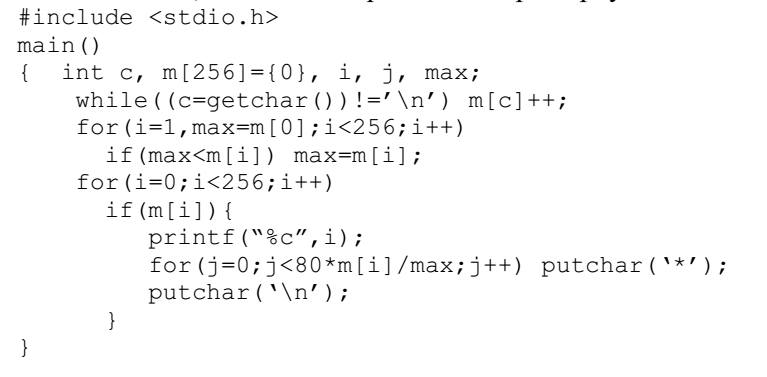
\includegraphics[scale=0.5]{images/lec02-pic11.png}
\end{figure}
\end{frame}

\end{document}
